\newpage
\begin{appendices}
\section{Evaluation of Existing Machine-learning based Name Generation Approaches for Generating Test Names}
\label[appendix]{sec:pilot-study}

Recent machine-learning based approaches (e.g.,~\cite{alon2018code2seq,alon2019code2vec}) performed significantly better on method and class name generation than previous approaches (e.g.,~\cite{allamanis2015suggesting,zhang2016towards}).
%
However, it is unknown how well these machine-learning based approaches would work in the context of generating names for unit tests.
%
To evaluate their performance on that, we conducted a pilot study to check if they can perform well on generating descriptive test names.
%
This pilot study is based on two randomly selected sets of tests from \num{11} open source projects on Github.
%
Judging by the outcome of this study, we believe it is necessary to build a new test name generation approach that focuses on developer need (i.e., based on what makes the test unique among its siblings).


\subsection{Considered Name Generations Approaches}

%TODO[fixed] What are the ML techniques?  Why these ones?  How are they different?
As the state-of-the-art work on the topic of abstracting code to use it for name generation, \citeauthor{alon2018code2seq} proposed a series of novel approaches on representing code snippets as compositional paths or continuous distributed vectors~\cite{alon2018code2seq,alon2019code2vec}.
%
After an initial review of the results of their approaches, their generated test names basically outperformed every existing name generation technique as far as we know~\cite{arcuri2014automated,ghafari2015automatically,pollock2010natural,pradel2018deepbugs,zhang2016towards,host2009debugging,schafer2008sound,allamanis2015suggesting,daka2017generating}.
%
The difference between the two approaches is that \texttt{Code2seq} encodes a code snippet to a set of compositional paths, and \texttt{Code2vec} encodes a code snippet to a fixed-length continuous vector.
%
Nonetheless, both of their approaches can make accurate prediction of Java method names.

\subsection{Considered Unit Tests}

\begin{table}[t]
\centering
\caption{Experimental Subjects.}
\begin{tabular}
{
  l
  l
  S[table-format=5.1]
  S[table-format=5.1]
}
\toprule
\multicolumn{1}{c}{\textbf{Project}} &
\multicolumn{1}{c}{\textbf{Version}} & 
\multicolumn{1}{c}{\textbf{LoC}} &
\multicolumn{1}{c}{\textbf{\# Tests}}
\\
\midrule
 Guice             & 9b371d3 &  183049  & 1280   \\
 Moshi             & dbed99d  &  22168  & 716   \\
 Picasso           & a087d26  &  11006  & 229  \\
 Fastjson          & e05f1f9  &  195511  & 4950   \\
 Guava             & 368c337  &  400801  & 13962  \\
 Mockito           & 22c82dc   &  59839 & 2145   \\
 Socket.io-client  & 661f1e7  &  9478  & 85  \\
 Scribejava        & ea42bc9  &  15184  & 110   \\
 ExoPlayer         & 79da521  &  172148  & 1510   \\
 Javapoet          & e9460b8  &  10755  & 302   \\
 Barbecue          & 44a8632  &  10760  & 170   \\
\bottomrule
\end{tabular}
\label{tab:subjectsForPilot}
\end{table}


To gather the tests we examined in our study, we started with the \num{11} Java projects \footnote{Same projects in the empirical study} shown in~\cref{tab:subjectsForPilot}.
%
In the table, the first column, \emph{Name}, shows the name of the project; the second column, \emph{Version}, shows the version of the project (either as a Git hash or version number); the fourth column, \emph{LoC}, shows the number of non-comment, non-blank lines of code as computed by SLOC count~\cite{nguyen2007sloc}; and the final column, \emph{\# Tests}, shows the number of unit tests in the project. In total, these \num{11} projects contain \num{25459} unit tests.
%
The first ten projects were randomly selected from the top \num{50} Java projects hosted on Github~\cite{top50projects}.
%
Because these projects encompass a variety of domains (e.g., JavaPoet is a library for generating Java programmatically and ExoPlayer is a media player for Android) and have many contributors (e.g., Moshi’s test suite contains contributions from \num{8} different people), their tests are more likely to be representative of tests in general which helps mitigate a potential threat to validity.
%
In addition, we also included Barbecue, a commonly used subject in the testing literature (e.g.,~\cite{zhang2015automatically, zhang2016towards,wu2020pattern}).
%
\num{15400} tests were randomly selected from different test classes under different projects to evaluate both \texttt{Code2seq} and \texttt{Code2vec}.

% [changed]WHy different number?

To investigate this research question, we run each corresponding set of tests on \texttt{Code2seq} and \texttt{Code2vec} and collected the generated test names as the data for dicussion.
%
Both \texttt{Code2seq} and \texttt{Code2vec} were run on a MacBook Pro (2.4GHz Intel i5 processor and 8GB RAM) with MacOS Mojave \footnote{Same machine in the empirical study}, Tensorflow 1.13.1 and Tensorflow 2.0.0, respectively.
%
And it took roughly \num{25} hours to both configure necessary environment and generating names for tests.


\subsection{Data and Discussion}

% Example figure for each... 
% Individually, names may look ``OK''.
% However, 

\begin{figure}[t]
\centering
\begin{subfigure}[b]{1.0\textwidth}
\centering
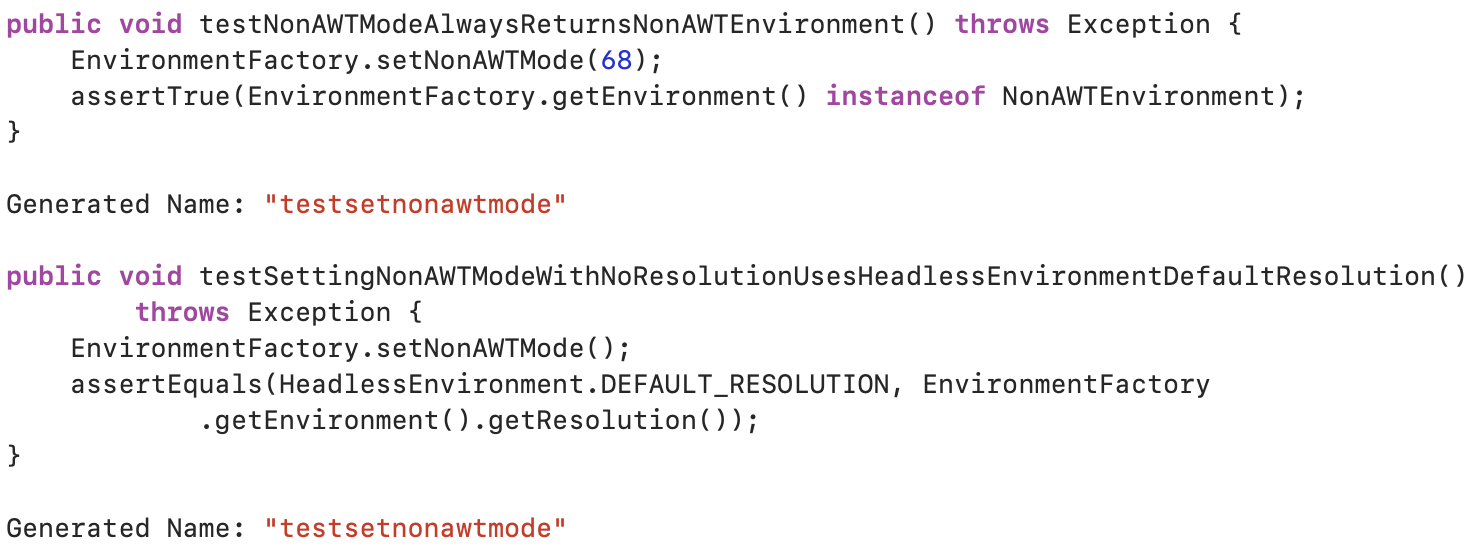
\includegraphics[scale=0.5]{figures/dup1.png}
\caption{Generated names by \texttt{Code2seq}.}
\label{fig:generated1}
\end{subfigure}\\
\vspace{0.2cm}
\begin{subfigure}[b]{0.5\textwidth}
\centering
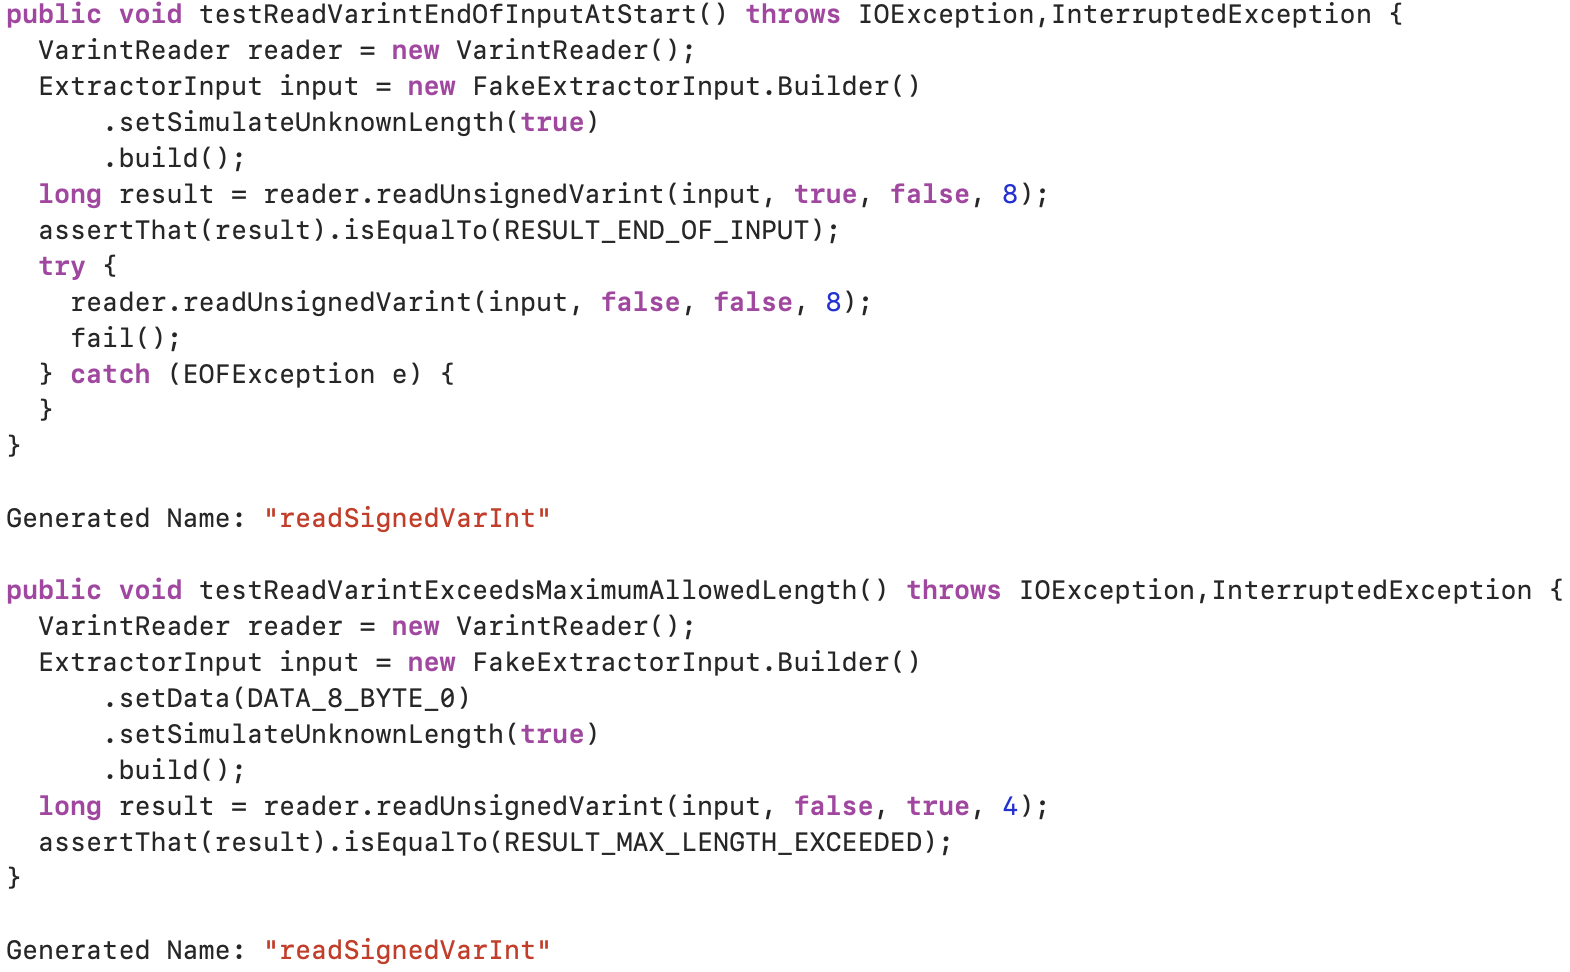
\includegraphics[scale=0.5]{figures/dup2.png}
\caption{Generated names by \texttt{Code2vec}.}
\label{fig:generated2}
\end{subfigure}
\caption{Example of generated names.}
\label{fig:duplicate-names}
\end{figure}


In~\cref{fig:generated1}, it shows two test names generated for Scribejava by using \texttt{Code2seq}.
%
For example, \texttt{extract\-With\-Empty\-Response} is generated for \texttt{should\-Throw\-Exception\-If\-Response\-Is\-Empty\-String}.
%
In~\cref{fig:generated2}, it shows two test names generated for ExoPlayer by using \texttt{Code2vec}.
%
For another example, \texttt{accumulate} is generated for \texttt{test\-Merge}.
%
Individually, these generated names might look to be acceptable.
%
However, each generated name has multiple duplicates in its related test class.
%
For instance, \texttt{extract\-with\-empty\-response} is repeated \num{3} times, and \texttt{accumulate} is repeated \num{4} times, in their corresponding test classes.
%
Therefore, they are useless in practice as duplicate names are not possible and, even if they were, they would not serve the goal of helping developers comprehend the purposes of their tests.



We collected and analyzed the generated test names from both \texttt{Code2seq} and \texttt{Code2vec}.
%
If there are many generated test names that are repeated at least once in its associated test class, it is necessary to develop a uniqueness-focused approach to solve the problem of duplication.
%
The collected data is shown in a shared document~\cite{CodeResult}.
%
It shows hundreds or thousands of duplicate names were generated for each project during their name generation process. 
%
For example, \texttt{Code2seq} produced \num{240} duplicate test names for ExoPlayer, and \num{57} out of \num{187} test classes in ExoPlayer contain more than one duplicate names.
%
For another example, \texttt{Code2vec} produced \num{1161} duplicate test names for Guava, and \num{209} out of \num{458} test classes in Guava contain more than one duplicate names.
%
Both state-of-the-art approaches produced a significant number of duplicate names when performing their automated name generation on unit tests.
%
This result indicates there is a need to develop a uniqueness-focused approach that can extract unique attributes of tests to generate descriptive names.


\end{appendices}